\newif\ifstandalone
%\standalonetrue

\ifstandalone
\documentclass[12pt,a4wide]{article}

% Andrea's packages
\usepackage{a4wide,amsmath,amssymb,graphicx,color}  

% Alexander's packages 
\usepackage[dvipsnames]{xcolor}
\usepackage{listings,enumitem,calc,hyperref,caption,mmacells} 
\lstset{basicstyle=\small\ttfamily,breaklines=true,breakatwhitespace=true}
\allowdisplaybreaks

\begin{document}
\fi

\section{User's manual} \label{sec:manual} 

This section describes the most important technical details of H1jet, including its installation and usage. 

\subsection{Installation} 
A tarball with the source files of H1jet can be obtained from ref.\ \cite{bib:h1jet}. Unpacking will result in a main directory \texttt{H1jet} with the following subdirectories: 
\begin{description}[labelindent=\parindent, labelwidth =\widthof{\bfseries9999}, leftmargin = !]
	\item[\texttt{bin} :] contains the executable program \texttt{h1jet} after compilation, as well as the Python 3 helper scripts \texttt{PlotH1jet.py} and \texttt{DressUserAmpCode.py}. 
	\item[\texttt{src} :] source files. 
\end{description}
The \texttt{README.md} file contains information on installation and usage. \\

In the main directory, run the configure script: 
\begin{lstlisting}
	$ ./configure [options] 
\end{lstlisting}
It will attempt to find a Fortran compiler (\texttt{gfortran} or \texttt{ifort}), as well as the dependencies on your machine. If you wish to specify a specific compiler and/or compiler flags, you can do so with the options \texttt{./configure FC=<compiler>} and \texttt{./configure FFLAGS=<flags>}. H1jet has a number of external dependencies which it must be linked to: 
\begin{itemize}
	\item LHAPDF \cite{bib:lhapdf}: Provides the PDF sets for H1jet. 
	\item \textsc{HOPPET} \cite{bib:hoppet}: For QCD DGLAP evolution of PDFs. 
	\item \textsc{Chaplin} \cite{bib:chaplin}: For complex harmonic polylogarithms. 
\end{itemize} 
For the \textsc{Chaplin} library, it may be necessary to explicitly state the path to the library files with:
\begin{lstlisting}
	$ ./configure LDFLAGS=-L/path/to/chaplin/lib 
\end{lstlisting}
To compile with a custom user interface: 
\begin{lstlisting}
	$ ./configure USERFILE=/path/to/custom/user_interface.f90  
\end{lstlisting}
See Section \ref{sec:newprocs} below for the implementation of custom user-specified amplitudes. \\ 
To install in a specific location: 
\begin{lstlisting}
	$ ./configure --prefix=/path/to/installation 
\end{lstlisting}
The default installation path is the main \texttt{H1jet}-directory. \\ 
The configure script will generate the \texttt{Makefile}. \\ 
To compile H1jet with the generated \texttt{Makefile}, run: 
\begin{lstlisting}
	$ make [options] 
\end{lstlisting}
This command takes the following options: \texttt{make clean} will delete all module and object files; \texttt{make distclean} will delete all module and object files as well as the executable \texttt{h1jet}. \\ 

After compilation, the \texttt{bin}-directory can then be added to the user's \texttt{PATH} environment variable. Alternatively, if the user has specified an install directory with the \texttt{--prefix} option, the executable can be installed with: 
\begin{lstlisting}
	$ make install  
\end{lstlisting}
The executable \texttt{h1jet} can then be found in the \texttt{bin}-directory at the path specified by \texttt{--prefix}. 

\subsection{Usage} 
After compilation, H1jet can be run from the \texttt{bin}-directory with: 
\begin{lstlisting}
	$ ./bin/h1jet [options]  
\end{lstlisting}
The following standard UNIX options are available: 
\begin{description}[labelindent=\parindent, labelwidth =\widthof{\bfseries9999999999999999999999}, leftmargin = !] 
	\item[\texttt{-h, --help}] Display the help message along with all possible options. 
	\item[\texttt{-v, --version}] Display the version of the installed H1jet. 
\end{description}
H1jet will display the requested information and then terminate. 

To direct the output to a file, use the option:
\begin{description}[labelindent=\parindent, labelwidth =\widthof{\bfseries9999999999999999999999}, leftmargin = !] 
	\item[\texttt{-o, --out <file>}] Direct the output to \texttt{<file>}. 
\end{description}
The physics process can be selected with: 
\begin{description}[labelindent=\parindent, labelwidth =\widthof{\bfseries9999999999999999999999}, leftmargin = !] 
	\item[\texttt{--proc <arg>}] Specify the process. Arguments: \vspace{-2mm} 
	\begin{description}[labelwidth =\widthof{\bfseries99999}, leftmargin = !] 
		\item[\texttt{H}] $pp/p\bar{p} \rightarrow H + \text{jet}$ (default). 
		\item[\texttt{bbH}] $b\bar{b} \rightarrow H + \text{jet}$. 
		\item[\texttt{Z}] $pp/p\bar{p} \rightarrow Z + \text{jet}$. 
		\item[\texttt{user}] User specified process. See Section \ref{sec:newprocs} below for implementation. 
	\end{description}
\end{description}
Depending on the process selected, there exists different relevant options. 

\subsubsection{General Options}
The options listed here apply to all processes. 
\begin{description}[labelindent=\parindent, labelwidth =\widthof{\bfseries9999999999999999999999}, leftmargin = !] 
	\item[\texttt{--collider <arg>}] Specify the collider type. \\ Arguments: \texttt{pp} (default), \texttt{ppbar}. 
	\item[\texttt{--roots <value>}] Center-of-mass energy in [GeV]. \\ Default: 13000 GeV. 
	\item[\texttt{--pdf\_name <arg>}] Specify the PDF set name from LHAPDF. \\ Please make sure that the specified PDF set is available in the local installation of LHAPDF. \\ Default: \texttt{MSTW2008nlo68cl}. 
	\item[\texttt{--pdf\_mem <value>}] Integer value specifying the PDF member. \\ Default: 0. 
	\item[\texttt{--scale\_strategy <arg>}] Set the scale strategy, i.e. the dynamic $\mu = \mu_R = \mu_F$ value. Arguments: \vspace{-2mm} 
	\begin{description}[labelwidth =\widthof{\bfseries99999}, leftmargin = !] 
		\item[\texttt{M}] $\mu_R = \mu_F = M$. 
		\item[\texttt{HT}] $\mu_R = \mu_F = p_T + \sqrt{p_T^2 + M^2}$ (default). 
		\item[\texttt{MT}] $\mu_R = \mu_F = \sqrt{p_T^2 + M^2}$. 
	\end{description} \vspace{-1mm} 
	Where the mass $M$ is given by option \texttt{--mH} for processes \texttt{H} and \texttt{bbH}, option \texttt{--mZ} for process \texttt{Z}, and option \texttt{--mass} for process \texttt{user}. 
	\item[\texttt{--xmur <value>}] Additional factor $x_{\mu_R}$ for the renormalisation scale, multiplied to the choice from \texttt{--scale\_strategy}. \\ Default: 0.5. 
	\item[\texttt{--xmuf <value>}] Additional factor $x_{\mu_F}$ for the factorisation scale, multiplied to the choice from \texttt{--scale\_strategy}. \\ Default: 0.5. 
	\item[\texttt{--nbins <value>}] Number of histogram bins in the output. \\ Default: 400. 
	\item[\texttt{--log}] Enables logarithmic $x$-axis of the histogram, i.e.\ logarithmic bins and $p_{T}$. Remember to set option \texttt{--ptmin} to a non-zero value. 
	\item[\texttt{--ptmin <value>}] Minimum $p_{T}$ value [GeV]. \\ Default: 0 GeV. 
	\item[\texttt{--ptmax <value>}] Maximum $p_{T}$ value [GeV]. \\ Default: 4000 GeV. 
	\item[\texttt{--accuracy <value>}] The desired integration accuracy. \\ Default: 0.001. 
\end{description}

\subsubsection{Relevant Options for Process: \texttt{H}}
If process \texttt{H}, i.e.\ 
\begin{equation}
	pp/p\bar{p} \rightarrow H + \text{jet}
\end{equation}
has been selected, then the following options are relevant: 
\begin{description}[labelindent=\parindent, labelwidth =\widthof{\bfseries9999999999999999999999}, leftmargin = !] 
	\item[\texttt{--mH <value>}] Higgs mass, $m_H$ [GeV]. \\ Default: 125 GeV. 
	\item[\texttt{--mW <value>}] W boson mass, $m_W$ [GeV]. \\ Default: 80.385 GeV. 
	\item[\texttt{--mZ <value>}] Z boson mass, $m_Z$ [GeV]. \\ Default: 91.1876 GeV.
	\item[\texttt{--mt <value>}] Top quark mass, $m_t$ [GeV]. \\ Default: 173.5 GeV. 
	\item[\texttt{--mb <value>}] On-shell bottom quark mass, $m_b^{\text{OS}}$ [GeV]. \\ Default: 4.65 GeV. 
	\item[\texttt{--yt <value>}] Top Yukawa factor [GeV]. \\ Default: 1. 
	\item[\texttt{--yb <value>}] Bottom Yukawa factor [GeV]. \\ Default: 1. 
	\item[\texttt{--GF <value>}] Fermi coupling constant, $G_F$ [GeV$^{-2}$]. \\ Default: $0.116638 \times 10^{-4}$ GeV$^{-2}$. 
\end{description}
Note that the Yukawa couplings are given by $y_q m_q / v$, where $y_q$ are the dimensionless factors specified by the options \texttt{--yt} and \texttt{--yb} above. \\ 

Note also that H1jet uses the $G_{\mu}$ scheme for the all electroweak parameters. Hence, the Higgs vacuum expectation value is given by $v = 1 / \sqrt{\sqrt{2} G_F}$, and the Weinberg angle is $\sin^2\left ( \theta_W \right ) = 1 - m_W^2 / m_Z^2$. \\ 

To consider a CP-odd Higgs instead, use the following option: 
\begin{description}[labelindent=\parindent, labelwidth =\widthof{\bfseries9999999999999999999999}, leftmargin = !] 
	\item[\texttt{--cpodd}] Toggle for calculation of CP-odd Higgs instead. 
\end{description}
The coupling between the CP-odd Higgs and the SM top quark is: 
\begin{equation}
   \mathcal{L} \supset i \tilde{\kappa}_t \frac{m_t}{v} \bar{t} \gamma_5 t h
\end{equation}
where the implementation in H1jet uses $\tilde{\kappa}_t = 1$. 

\paragraph{Top-partner} 
To include a top-partner $T$ in the quark loops, it will be necessary to set the top-partner mass $m_T$ to a non-zero value by using the \texttt{--mtp} option. 

The SM top Yukawa coupling factor can be modified by the mixing angle, 
\begin{equation}
   y_t \rightarrow y_t \cos^2\theta_T \,, 
\end{equation} 
where $y_t$ is the Yukawa factor set by option \texttt{--yt}. 

The top-partner Yukawa coupling factor will likewise be modified 
\begin{equation}
   y_T \rightarrow y_T \sin^2\theta_T \,. 
\end{equation} 
with $y_T$ set by \texttt{--ytp}. 

The top-partner specific options are: 
\begin{description}[labelindent=\parindent, labelwidth =\widthof{\bfseries9999999999999999999999}, leftmargin = !] 
	\item[\texttt{--mtp <value>}] Top-partner mass, $m_{T}$ [GeV]. \\ Default: 0 GeV. 
	\item[\texttt{--ytp <value>}] Top-partner Yukawa factor, $y_T$. \\ Default: 1. 
	\item[\texttt{--sth2 <value>}] Top-partner mixing angle, $\sin^2 \theta_T$. \\ Default: 0. 
\end{description} 
The top-partner can also be considered in the composite Higgs models as described in \cite{}. There are four different models, $\textbf{M1}_{\textbf{5}}$, $\textbf{M1}_{\textbf{14}}$, $\textbf{M4}_{\textbf{5}}$, and $\textbf{M4}_{\textbf{14}}$, which modifies the Yukawa coupling factors in the following way: 
\begin{eqnarray}
	\textbf{M1}_{\textbf{5}}: && \hspace{5mm} \begin{array}{l} 
		y_b \rightarrow y_b c_\varepsilon \\ 
		y_t \rightarrow y_t c_\varepsilon \cos^2 \theta_T \\ 
		y_T \rightarrow y_T c_\varepsilon \sin^2 \theta_T \\ 
		\tilde{y}_b = \tilde{y}_t = \tilde{y}_T = 0 
	\end{array} \\ \nonumber \\ 
	\textbf{M1}_{\textbf{14}}: && \hspace{5mm} \begin{array}{l} 
		y_b \rightarrow y_b \frac{2 c_\varepsilon^2 - 1}{c_\varepsilon} \\ 
		y_t \rightarrow y_t \frac{2 c_\varepsilon^2 - 1}{c_\varepsilon} \cos^2\theta_T  \\ 
		y_T \rightarrow y_T \frac{2 c_\varepsilon^2 - 1}{c_\varepsilon} \sin^2\theta_T  \\ 
		\tilde{y}_b = \tilde{y}_t = \tilde{y}_T = 0 
	\end{array} \\ \nonumber \\ 
	\textbf{M4}_{\textbf{5}}: && \hspace{5mm} \begin{array}{l} 
		y_b \rightarrow y_b c_\varepsilon \\ 
		y_t \rightarrow y_t c_\varepsilon \left ( \cos^2\theta_R - \frac{s_\varepsilon^2}{1 + c_\varepsilon^2} \left ( \cos^2\theta_L - \cos^2\theta_R \right ) \right ) \\ 
		y_T \rightarrow y_T c_\varepsilon \left ( \sin^2\theta_R - \frac{s_\varepsilon^2}{1 + c_\varepsilon^2} \left ( \sin^2\theta_L - \sin^2\theta_R \right ) \right ) \\ 
		\tilde{y}_b = 0 \\
		\tilde{y}_t = \frac{4 c_\varepsilon s_\varepsilon}{\sqrt{2(1 + c_\varepsilon^2)}} \text{Im}(c_1) \sin\theta_R \cos\theta_R \\ 
		\tilde{y}_T = -\tilde{y}_t 
	\end{array} \\ \nonumber \\ 
	\textbf{M4}_{\textbf{14}}: && \hspace{5mm} \begin{array}{l} 
		y_b \rightarrow y_b \frac{2 c_\varepsilon^2 - 1}{c_\varepsilon} \\ 
		y_t \rightarrow y_t \left ( \frac{(2 c_\varepsilon^2 - 1)}{c_\varepsilon} \cos^2\theta_R - \frac{s_\varepsilon^2 c_\varepsilon (8 c_\varepsilon^2 - 3)}{1 - 3 c_\varepsilon^2 + 4 c_\varepsilon^4} \left ( \cos^2\theta_L - \cos^2\theta_R \right ) \right ) \\ 
		y_T \rightarrow y_T \left ( \frac{(2 c_\varepsilon^2 - 1)}{c_\varepsilon} \sin^2\theta_R - \frac{s_\varepsilon^2 c_\varepsilon (8 c_\varepsilon^2 - 3)}{1 - 3 c_\varepsilon^2 + 4 c_\varepsilon^4} \left ( \sin^2\theta_L - \sin^2\theta_R \right ) \right )) \\ 
		\tilde{y}_b = 0 \\
		\tilde{y}_t = \frac{4 s_\varepsilon (1 - 2 s_\varepsilon^2)}{\sqrt{2(1 - 3 c_\varepsilon^2 + 4 c_\varepsilon^4)}} \text{Im}(c_1) \sin\theta_R \cos\theta_R \\ 
		\tilde{y}_T = -\tilde{y}_t 
	\end{array}
\end{eqnarray}
where the $\tilde{y}$'s are the CP-odd couplings, and, 
\begin{equation}
	s_\varepsilon = \frac{v}{f} \,, \hspace{7 mm} \text{ and } \hspace{7 mm} c_\varepsilon = \sqrt{1 - s_\varepsilon^2} \,,
\end{equation}
and where the $\theta_R$ and $\theta_L$ mixing angles are related to $\theta_T$, 
\begin{eqnarray}
	& \theta_R = \theta_T \,, \nonumber \\ 
	& \tan^2\theta_L = \frac{m_T^2}{m_t^2} \tan^2\theta_T \,, \\ 
	& \sin^2\theta_L = \frac{1}{1 + \tan^2\theta_L}, \hspace{7 mm} \cos^2\theta_L = 1 - \sin^2\theta_L \,. \nonumber  
\end{eqnarray}
The composite Higgs top-partner model specific options are: 
\begin{description}[labelindent=\parindent, labelwidth =\widthof{\bfseries9999999999999999999999}, leftmargin = !] 
	\item[\texttt{--model <arg>}] Specify the top-partner model. Arguments: \vspace{-2mm} 
	\begin{description}[labelwidth =\widthof{\bfseries999999}, leftmargin = !] 
		\item[\texttt{M1\_5}] $\textbf{M1}_{\textbf{5}}$, with a light top-partner transforming as a $\textbf{1}_{\textbf{2/3}}$ of $\text{SO}(4)$, and the SM top-bottom doublet embedded in a $\textbf{5}$ of $\text{SO}(5)$ (default). 
		\item[\texttt{M1\_14}] $\textbf{M1}_{\textbf{14}}$, with a light top-partner transforming as a $\textbf{1}_{\textbf{2/3}}$ of $\text{SO}(4)$, and the SM top-bottom doublet embedded in a $\textbf{14}$ of $\text{SO}(5)$. 
		\item[\texttt{M4\_5}] $\textbf{M4}_{\textbf{5}}$, with a light top-partner transforming as a $\textbf{4}_{\textbf{2/3}}$ of $\text{SO}(4)$, and the SM top-bottom doublet embedded in a $\textbf{5}$ of $\text{SO}(5)$. 
		\item[\texttt{M4\_14}] $\textbf{M4}_{\textbf{5}}$, with a light top-partner transforming as a $\textbf{4}_{\textbf{2/3}}$ of $\text{SO}(4)$, and the SM top-bottom doublet embedded in a $\textbf{14}$ of $\text{SO}(5)$. 
	\end{description} \vspace{-1mm} 
	\item[\texttt{--imc1 <value>}] Imaginary part of the $c_1$ coefficient, $\text{Im}(c_1)$. \\ Default: 0.  
	\item[\texttt{--fscale <value>}] Top-partner confinement scale, $f$ [GeV]. \\ Default: 0 GeV. 
\end{description} 

\paragraph{Multiple top-partners models}
To include multiple top-partners in the quark loops, it will be necessary to specify an input file with the masses and Yukawa coupling factors for each top-partner. This can be done with the following option: 
\begin{description}[labelindent=\parindent, labelwidth =\widthof{\bfseries9999999999999999999999}, leftmargin = !] 
	\item[\texttt{-i, --i <file>}] Include input file with top-partner masses and Yukawas. See the file \texttt{SM.dat} for an example. 
\end{description} 
The first line of the input file should specify the number of top-partners, e.g.: 
\begin{lstlisting}
	nqmax: 2 
\end{lstlisting}
This should be followed by \texttt{nqmax} number of lines -- one for each top-partner -- in the format of four numbers specifying the mass, $\kappa$, $\tilde{\kappa}$, and loop approximation, in that order. For example, for a SM top quark: 
\begin{lstlisting}
	173.5 1.0 0.0 1 
\end{lstlisting}
with mass $173.5$ GeV, $\kappa = 1$, $\tilde{\kappa} = 0$, and the loop approximation set to $1$. \\ 

The dimensionless Yukawa coupling factors $\kappa$ and $\tilde{\kappa}$ are the CP-even and CP-odd couplings respectively, with the following Lagrangian: 
\begin{equation}
	\mathcal{L} \supset -m_T \bar{T}T + \kappa \frac{m_T}{v} \bar{T}T h + i \tilde{\kappa} \frac{m_T}{v} \bar{T} \gamma_5 T h 
\end{equation}
for a top-partner $T$. \\ 

The integer value specifying the loop approximations can take the following values: 
\begin{description}[labelindent=3\parindent, labelwidth =\widthof{\bfseries9999}, leftmargin = !] 
	\item[$0$] Small mass limit for fermions. 
	\item[$1$] Full mass limit for fermions. 
	\item[$2$] Large mass limit for fermions. 
	\item[$3$] Full mass limit for scalars. 
	\item[$4$] Large mass limit for scalars. 
\end{description}
See Section \ref{sec:loopapprox} for more information on the loop approximations. 

\paragraph{MSSM}
To include the MSSM stops $\tilde{t}_1$ and $\tilde{t}_2$ in the quark loops, it will be necessary to set the first stop mass $m_{\tilde{t}_1}$ to a non-zero value by using the \texttt{--mst} option. The second stop mass is then given by 
\begin{equation}
	m_{\tilde{t}_2} = \sqrt{m_{\tilde{t}_1}^2 + \Delta m^2} 
\end{equation}
where $\Delta m$ is set with the \texttt{--delta} option. 

The stop Yukawa coupling factors will be given by: 
\begin{equation}
   y_{\tilde{t}_1} = \frac{m_t^2}{m_{\tilde{t}_1}^2} \left [ \alpha_1 \cos^2 \theta_{\tilde{t}} + \alpha_2 \sin^2 \theta_{\tilde{t}} + 2 - \frac{\Delta m^2}{2 m_t^2} \sin^2\left ( 2 \theta_{\tilde{t}} \right ) \right ] \,,
\end{equation} 
\begin{equation}
   y_{\tilde{t}_2} = \frac{m_t^2}{m_{\tilde{t}_2}^2} \left [ \alpha_1 \sin^2 \theta_{\tilde{t}} + \alpha_2 \cos^2 \theta_{\tilde{t}} + 2 + \frac{\Delta m^2}{2 m_t^2} \sin^2\left ( 2 \theta_{\tilde{t}} \right ) \right ] \,, 
\end{equation} 
where 
\begin{equation}
   \alpha_1 = \frac{m_Z^2}{m_t^2} \cos \left ( 2 \beta \right ) \left [ 1 - \frac{4}{3} \sin^2\theta_W \right ] \,, 
\end{equation} 
\begin{equation}
   \alpha_2 = \frac{4}{3} \frac{m_Z^2}{m_t^2} \cos \left ( 2 \beta \right ) \sin^2\theta_W \,. 
\end{equation} 
Note that $m_t$, $m_Z$, and $\sin^2\theta_W$ can be set with the \texttt{--mt}, \texttt{--mZ}, and \texttt{--sinwsq} options respectively, while $\sin^2 \theta_{\tilde{t}}$ and $\tan\beta$ are MSSM specific options and can be set with the \texttt{--sth2} and \texttt{--tbeta} options. 

All of the MSSM specific options are: 
\begin{description}[labelindent=\parindent, labelwidth =\widthof{\bfseries9999999999999999999999}, leftmargin = !] 
	\item[\texttt{--mst <value>}] MSSM stop mass, $m_{\tilde{t}}$ [GeV]. \\ Default: 0 GeV. 
	\item[\texttt{--delta <value>}] MSSM stop mass separation $\Delta m$ [GeV]. \\ Default: 0 GeV. 
	\item[\texttt{--sth2 <value>}] Stop mixing angle, $\sin^2 \theta_{\tilde{t}}$. \\ Default: 0. 
	\item[\texttt{--tbeta <value>}] Ratio of VEVs in MHDMs, $\tan\beta$. \\ Default: 0. 
\end{description}
Note that the top partner mass $m_{T}$ and MSSM stop mass $m_{\tilde{t}_1}$ can not both be set non-zero at the same time. 

The MSSM implementation described here is in the decoupling limit, $m_A \gg m_Z$, of ref.\ \cite{bib:mssm1} and \cite{bib:mssm2}. 

\subsubsection{Relevant Options for Process: \texttt{bbH}}
If process \texttt{bbH}, i.e.\ 
\begin{equation}
	b\bar{b} \rightarrow H + \text{jet}
\end{equation}
has been selected, then the following options are relevant: 
\begin{description}[labelindent=\parindent, labelwidth =\widthof{\bfseries9999999999999999999999}, leftmargin = !] 
	\item[\texttt{--mH <value>}] Higgs mass, $m_H$ [GeV]. \\ Default: 125 GeV. 
	\item[\texttt{--GF <value>}] Fermi coupling constant, $G_F$ [GeV$^{-2}$]. \\ Default: $0.116638 \times 10^{-4}$ GeV$^{-2}$. 
	\item[\texttt{--mbmb <value>}] $\overline{\text{MS}}$ bottom quark mass, $m_b^{\overline{\text{MS}}}$ [GeV]. \\ Default: 4.18 GeV. 
\end{description}

\subsubsection{Relevant Options for Process: \texttt{Z}}
If process \texttt{Z}, i.e.\ 
\begin{equation}
	pp/p\bar{p} \rightarrow Z + \text{jet}
\end{equation}
has been selected, then the following options are relevant: 
\begin{description}[labelindent=\parindent, labelwidth =\widthof{\bfseries9999999999999999999999}, leftmargin = !] 
	\item[\texttt{--mZ <value>}] Z boson mass, $m_Z$ [GeV]. \\ Default: 91.1876 GeV.
	\item[\texttt{--mW <value>}] W boson mass, $m_W$ [GeV]. \\ Default: 80.385 GeV. 
	\item[\texttt{--GF <value>}] Fermi coupling constant, $G_F$ [GeV$^{-2}$]. \\ Default: $0.116638 \times 10^{-4}$ GeV$^{-2}$. 
\end{description}

\subsubsection{Relevant Options for Process: \texttt{user}}
In the case of process \texttt{user}, i.e.\ a custom user-specified process, any of the above physics options may be relevant if they are used in the custom amplitude code. The code will have to be inspected to determine this. The only built-in process-relevant option is: 
\begin{description}[labelindent=\parindent, labelwidth =\widthof{\bfseries9999999999999999999999}, leftmargin = !] 
	\item[\texttt{--mass <value>}] Relevant mass in the user specified process, $M$ [GeV]. Used in the scale choice and in the setup of kinematics. \\ Default: 0 GeV. 
\end{description}
Additional options may be added depending on the custom process/amplitude. See Section \ref{sec:newprocs} below for more details on the implementation of a custom process. 

\subsubsection{Loop Approximations} \label{sec:loopapprox} 
Small and large mass limits can be used as approximations for the quarks in the loop calculations. This requires some knowledge of the meaning of the approximations, hence this needs to be set by the user at compile time. 

In the file \texttt{input.f90} located in the \texttt{src}-directory, the subroutine \texttt{reset\_iloop\_array} can be found. This subroutine can be used by the user to set the \texttt{iloop\_array}, which is an array specifying the approximation used for each loop particle. The approximations that can be used are: 
\begin{description}[labelindent=3\parindent, labelwidth =\widthof{\bfseries9999999999999999999}, leftmargin = !] 
	\item[\texttt{iloop\_sm\_fermion}] Small mass limit for fermions. 
	\item[\texttt{iloop\_fm\_fermion}] Full mass limit for fermions. 
	\item[\texttt{iloop\_lm\_fermion}] Large mass limit for fermions. 
	\item[\texttt{iloop\_fm\_scalar}] Full mass limit for scalars. 
	\item[\texttt{iloop\_lm\_scalar}] Large mass limit for scalars. 
\end{description}
The size of the array must match the number of particles appearing in the loops. This should be checked by the user.  

Here is an example snippet of Fortran code which could appear in the \texttt{reset\_iloop\_array} subroutine, which sets the approximations for an effective theory with SM top and bottom quarks, and one infinitely heavy top-partner: 
\begin{lstlisting}[language=Fortran, 
                   keywordstyle=\color{Red},
                   stringstyle=\color{Green},
                   identifierstyle=\color{Blue},
                   showstringspaces=false]
    if (size(iloop_array) == 3) then
      iloop_array = (/ iloop_fm_fermion, iloop_fm_fermion, &
                     & iloop_lm_fermion /)
    else
      call wae_error('reset_iloop_array', 'Expected size of &
           & iloop_array is 3, whereas actual one is', &
           & intval = size(iloop_array))
    end if
\end{lstlisting}

\subsubsection{Output}
H1jet will print out a brief summary of the settings and parameters used, as well as the born-level cross-section $\sigma_0$, followed by the $\mathrm{d}\sigma/\mathrm{d}p_{T}$ and $\sigma(p_{T})$ for each $p_T$ bin. \\ 

The helper script \texttt{PlotH1jet.py} facilitates easy and quick plotting of the output from H1jet. The script requires Python 3 installed in order to run. Simply pipe the output from H1jet to the script: 
\begin{lstlisting}
	$ ./h1jet [options] | python PlotH1jet.py 
\end{lstlisting}
A resulting example plot with default settings in H1jet is shown in \autoref{fig:h1jetresult}. 

\begin{figure}[tbh] 
  \centering
  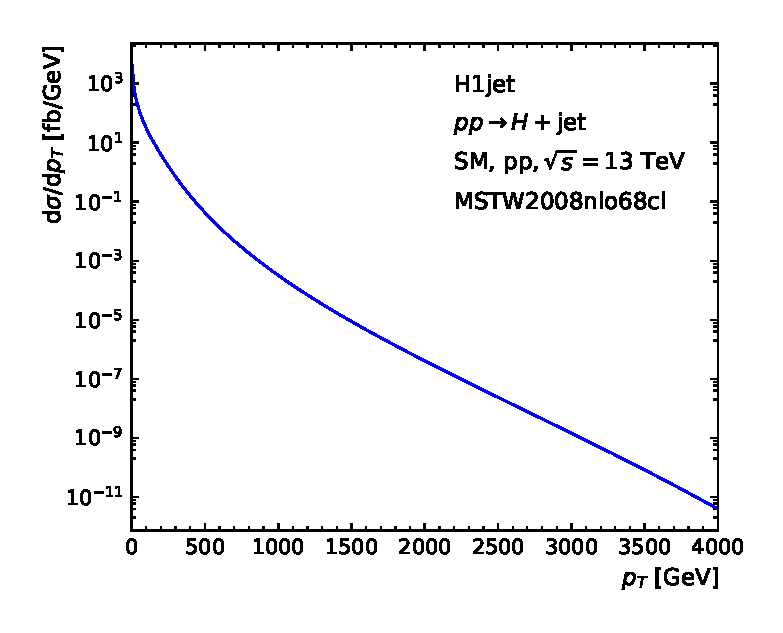
\includegraphics[width=0.6\linewidth]{figures/h1jetresult}
  \captionof{figure}{The $p_{T}$ distribution for the SM process $pp \rightarrow H + \text{jet}$ from H1jet with default settings.}
  \label{fig:h1jetresult}
\end{figure}

\newpage 

\section{Benchmarking} \label{sec:benchmarking} 
The various process implementations in H1jet have been compared to those of \textsc{SusHi} \cite{bib:sushi}, and have all been found to be in agreement. \\ 

The relative ratio between the H1jet result and the \textsc{SusHi} result for the $p_T$ distribution for the CP-odd Higgs are shown in \autoref{fig:cpoddratio}, and is found to be in agreement within the Monte Carlo error of \textsc{SusHi} for a large range of $p_T$ values. Smaller deviations may be due to the different handling of PDF evolution between the two programs. For low $p_T$ values, the larger deviation may be due to numerical issues in the calculation of the harmonic polylogarithms. Overall the agreement with \textsc{SusHi} is within $3 \times 10^{-4}$. \\ 

The low $p_T$ behaviour in \autoref{fig:cpoddratio} is due to possible numerical instability. The H1jet result can be further checked in the $p_{T} \rightarrow 0$ limit, by comparing it to the resummation expression, 
\begin{equation}
	\frac{\mathrm{d} \sigma}{\mathrm{d} p_T} \xrightarrow{p_T \rightarrow 0} \sigma_0 \left [ 4 C_A \frac{\alpha_s}{\pi} \frac{1}{p_T} \ln\left ( \frac{m_a}{p_T} \right ) + \mathcal{O} ( \alpha_s^2 ) \right ] \,, \label{eq:resum}
\end{equation}
where $\sigma_0$ is the total born-level cross-section for $gg \rightarrow h$. In \autoref{fig:cpoddresum}, we show $\frac{p_T}{\sigma_0} \left ( \frac{\mathrm{d} \sigma}{\mathrm{d} p_T} \right )$ with the first term of \autoref{eq:resum} subtracted, as a function of $\ln \frac{p_T}{m_h}$. For $p_T \rightarrow 0$ this goes nicely towards a constant as expected. 

\newpage 

\begin{figure}[h!] 
\centering
\begin{minipage}{.485\textwidth}
  \centering
  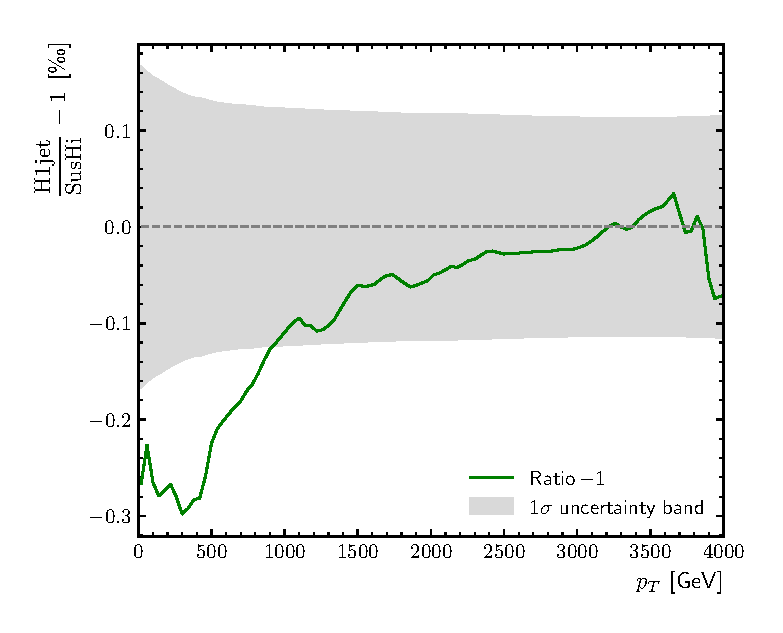
\includegraphics[width=\linewidth]{figures/CPoddratio}
  \captionof{figure}{The relative difference between the H1jet result and that of \textsc{SusHi} for the $p_T$ distribution for a CP-odd Higgs. The grey band indicates the Monte Carlo error of \textsc{SusHi}.}
  \label{fig:cpoddratio}
\end{minipage}%
\hfill% 
\begin{minipage}{.485\textwidth}
  \centering
  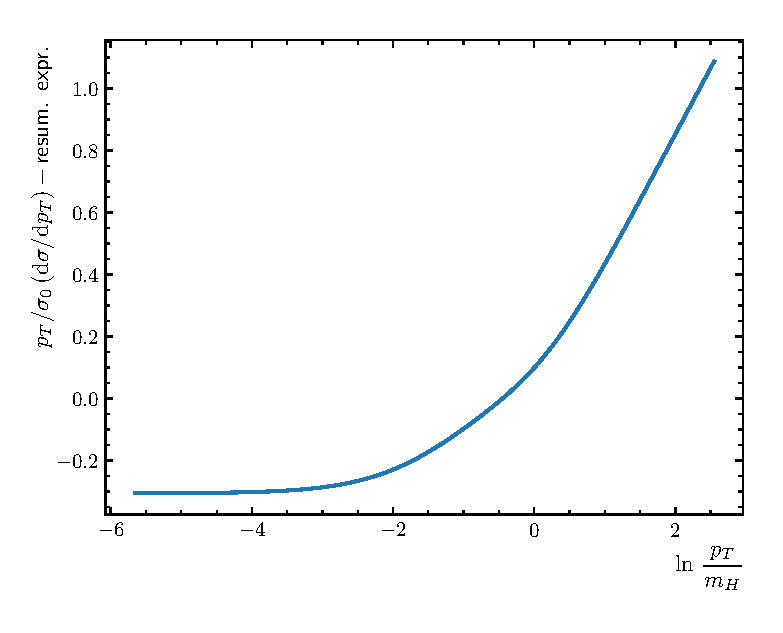
\includegraphics[width=\linewidth]{figures/CPoddresum}
  \captionof{figure}{The distribution $\frac{p_T}{\sigma_0} \left ( \frac{\mathrm{d} \sigma}{\mathrm{d} p_T} \right )$ with the first term of the $p_T$ resummation subtracted, as a function of $\ln \frac{p_T}{m_a}$. For low $p_T$ values it convergences to a constant value.}
  \label{fig:cpoddresum}
\end{minipage}
\end{figure}

The relative ratio between the H1jet and \textsc{SusHi} results for the MSSM are shown in \autoref{fig:mssmratio} and is within $2 \times 10^{-4}$. Again the low $p_T$ behaviour can be checked by comparing to the resummed expression in \autoref{fig:mssmresum}. 

\begin{figure}[h!] 
\centering
\begin{minipage}{.485\textwidth}
  \centering
  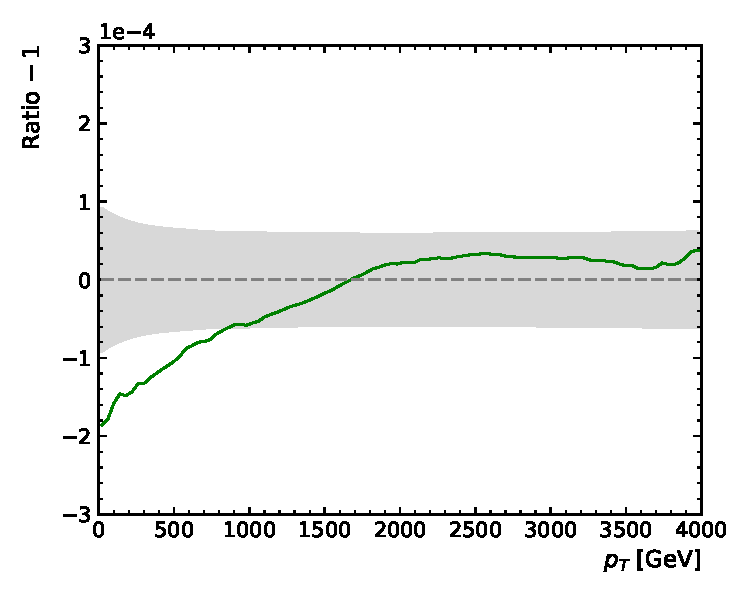
\includegraphics[width=\linewidth]{figures/MSSMratio}
  \captionof{figure}{The relative difference between the H1jet result and that of \textsc{SusHi} for the $p_T$ distribution in the MSSM. The grey band indicates the Monte Carlo error of \textsc{SusHi}.}
  \label{fig:mssmratio}
\end{minipage}%
\hfill% 
\begin{minipage}{.485\textwidth}
  \centering
  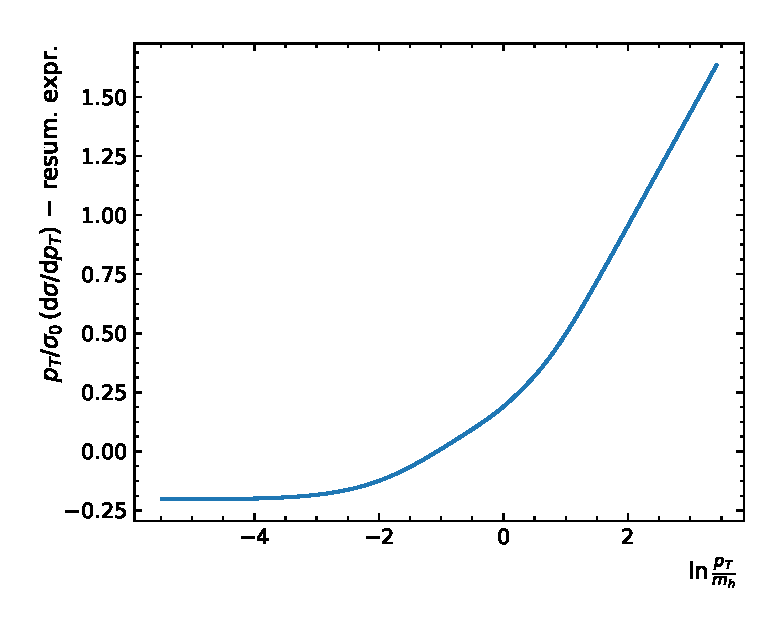
\includegraphics[width=\linewidth]{figures/MSSMresum}
  \captionof{figure}{The distribution $\frac{p_T}{\sigma_0} \left ( \frac{\mathrm{d} \sigma}{\mathrm{d} p_T} \right )$ with the first term of the $p_T$ resummation subtracted, as a function of $\ln \frac{p_T}{m_a}$. For low $p_T$ values it convergences to a constant value.}
  \label{fig:mssmresum}
\end{minipage}
\end{figure}

\newpage 

\section{Adding new processes to H1jet} \label{sec:newprocs} 
H1jet can be interfaced to use the squared matrix element evaluated from a custom Fortran code. The implementation may be most easily explained with a specific example. Please read this section carefully before attempting to use the interface. 

\subsection{Example: Axion-Like-Particle (ALP)}
We will present here a specific example of adding to H1jet the production of a light axion-like-particle (ALP) $a$ along with a jet. We will, for simplicity, only consider the gluon-fusion channel, 
\begin{equation}
    g g \rightarrow g a \,. 
\end{equation}
This is a tree-level process due to an effective ALP-gluon coupling, 
\begin{equation}
   \delta \mathcal{L}_a \supset -c_{\tilde{G}}\frac{a}{f_a} G_{\mu\nu}^{a} \tilde{G}^{a \mu\nu} \,. \label{eq:ggacoupling}
\end{equation}
The model and the \textsc{FeynRules} \cite{bib:feynrules} model files are described and provided in ref.\ \cite{bib:alp}. We will be using \textsc{FeynCalc} \cite{bib:feyncalc} to evaluate the amplitude from the model, so we will have to convert the \textsc{FeynRules} model to a \textsc{FeynArts} \cite{bib:feynarts} model in Mathematica: 
\begin{mmaCell}{Code}
<< FeynRules` 
\end{mmaCell}
\begin{mmaCell}{Code}
LoadModel["SM.fr", "alp_linear.fr", "alp_linear_operators.fr"];  
\end{mmaCell}
\begin{mmaCell}{Code}
WriteFeynArtsOutput[LSM + LALP, CouplingRename -> False]; 
\end{mmaCell}
The resulting \textsc{FeynArts} model files are written to a new directory \texttt{ALP\_linear\_FA}, which needs to be moved to the \textsc{FeynArts/Models} directory. Note that in the \textsc{FeynArts} model, the ALP field is called \texttt{S[4]} and the gluon fields are called \texttt{V[4]}. 

In a new Mathematica session, load \textsc{FeynCalc} with \textsc{FeynArts}: 
\begin{mmaCell}{Code}
$LoadAddOns = {"FeynArts"}; 
\end{mmaCell}
\begin{mmaCell}{Code}
<< FeynCalc` 
\end{mmaCell}
The \textsc{FeynArts/Models} directory can be located with: 
\begin{mmaCell}{Code}
$FeynArtsDir
\end{mmaCell}
First patch the \texttt{ALP\_linear\_FA} model with: 
\begin{mmaCell}{Code}
FAPatch[PatchModelsOnly -> True] 
\end{mmaCell}
This ensures that the model files works with \textsc{FeynCalc}. 

Then create the tree-level $2 \rightarrow 2$ topologies and insert the fields for our process: 
\begin{mmaCell}{Code}
tops = CreateTopologies[0, 2 -> 2];
\end{mmaCell}
\begin{mmaCell}{Code}
ins = InsertFields[tops, {V[4], V[4]} -> {V[4], S[4]}, InsertionLevel -> {Classes}, Model -> "ALP_linear_FA", GenericModel -> "ALP_linear_FA"];
\end{mmaCell}
It is possible to draw the Feynman diagrams for the process as a check: 
\begin{mmaCell}{Code}
Paint[ins, ColumnsXRows -> {2, 1}, Numbering -> Simple, SheetHeader -> None, ImageSize -> {512, 256}]; 
\end{mmaCell}
We will then set up the amplitude: 
\begin{mmaCell}{Code}
feynamp = CreateFeynAmp[ins];  
\end{mmaCell}
\begin{mmaCell}{Code}
amp = FCFAConvert[feynamp, IncomingMomenta -> {k1, k2}, OutgoingMomenta -> {k3, k4}, UndoChiralSplittings -> True, ChangeDimension -> 4, TransversePolarizationVectors -> {k1, k2, k3}, List -> False, SMP -> True, Contract -> True, DropSumOver -> True] 
\end{mmaCell}
While not strictly necessary, it is recommended to enable the \texttt{SMP} option. Any additional substitutions in the amplitude can be specified with the \texttt{FinalSubstitutions} option. 

We will then set up the kinematics: 
\begin{mmaCell}{Code}
FCClearScalarProducts[]; 
\end{mmaCell}
\begin{mmaCell}{Code}
SetMandelstam[s, t, u, k1, k2, -k3, -k4, 0, 0, 0, mA]; 
\end{mmaCell}
We introduce here a parameter \texttt{mA} for the ALP mass $m_a$. 

We can then square the amplitude: 
\begin{mmaCell}{Code}
ampsquared = Simplify[
  (TrickMandelstam[#1, {s, t, u, mA^2}] & )[
    (DoPolarizationSums[#1, k2, k1, ExtraFactor -> 1/2] & )[
      (DoPolarizationSums[#1, k1, k2, ExtraFactor -> 1/2] & )[ 
        (DoPolarizationSums[#1, k3, 0] & )[ 
          (SUNSimplify[#1, Explicit -> True, SUNNToCACF -> False] & )[
            FeynAmpDenominatorExplicit[(1 / (SUNN^2 - 1)^2) * (amp * ComplexConjugate[amp])]]]]]]] /. SUNN -> 3 
\end{mmaCell}
Setting the \texttt{SUNNToCACF} option in \texttt{SUNSimplify[]} to \texttt{False} is not necessary, nor is it necessary to fix \texttt{SUNN} to $3$. This can be handled by the dressing script and H1jet. 

Finally, we will write the amplitude as Fortran code to a file: 
\begin{mmaCell}{Code}
Write2["ALP_amp.f90", gg = ampsquared, FormatType -> FortranForm, FortranFormatDoublePrecision -> False] 
\end{mmaCell}
Note here that we specify the gluon-gluon channel with the \texttt{gg = ampsquared} input to the function. This is required for the subsequent dressing script to work properly. It is important to specify the $2$-particle initial state by using combinations of \texttt{g}, \texttt{u}, \texttt{d}, \texttt{c}, \texttt{s}, \texttt{b}, \texttt{ubar}, \texttt{dbar}, \texttt{cbar}, \texttt{sbar}, and \texttt{bbar}. One can also use \texttt{q} and \texttt{qbar} for all the light quarks and antiquarks respectively, i.e.\ $u$, $d$, $c$, and $s$. For example, \texttt{bbbar} will be the $b\bar{b}$ channel. \\ 

The generated Fortran code \texttt{ALP\_amp.f90} will have to be dressed by the Python helper script \texttt{DressUserAmpCode.py}: 
\begin{lstlisting}
	$ python DressUserAmpCode.py ALP_amp.f90 
\end{lstlisting}
This will produce a dressed Fortran code file by default called \texttt{user\_interface.f90}. 

The helper script has a help message which can be called with \texttt{-h} or \texttt{--help}. The name of the output file can be specified with the \texttt{-o} option. Multiple input Fortran files can be provided to the helper script. The full usage is: 
\begin{lstlisting}
	$ python DressFeynCalcCode.py [-h] [-o [OUTFILE]] inputfile [inputfile ...] 
\end{lstlisting}
The provided input Fortran code files does not necessarily have to be generated with \textsc{FeynCalc}. They can be generated by any other program or even be written by hand. \\ 

To use the new dressed custom Fortran code with H1jet, it is necessary to recompile H1jet with the custom Fortran code: 
\begin{lstlisting}
	$ ./configure USERFILE=/path/to/custom/user_interface.f90 
	$ make clean
	$ make 
\end{lstlisting}
Running \texttt{./h1jet --help} we see that three new additional options have been added: 
\begin{description}[labelindent=\parindent, labelwidth =\widthof{\bfseries9999999999999999999999}, leftmargin = !] 
	\item[\texttt{--c\_CGtil <value>}] The Wilson coefficient $c_{\tilde{G}}$ in \autoref{eq:ggacoupling}. 
	\item[\texttt{--c\_mA <value>}] The ALP mass, $m_a$. 
	\item[\texttt{--c\_fa <value>}] The ALP suppression scale $f_a$ in \autoref{eq:ggacoupling}. 
\end{description}
The leading \texttt{c\_} in the name stands for ``custom'' and is automatically added in order to avoid naming issues in the code. \\ 

The result from the ALP implementation in H1jet is shown in \autoref{fig:alpresult} and can be compared to the H1jet result for the CP-odd Higgs by using a single top quark in the loop with an infinite mass limit, resulting in an effective coupling between the CP-odd Higgs and the gluons. The respective ALP and CP-odd couplings are then related as such, 
\begin{equation}
	\frac{c_{\tilde{G}}^2}{f_a^2} = \frac{\alpha_s^2}{64 \pi^2 v^2} \,. 
\end{equation}
The comparison is shown in \ref{fig:alpratio} where we see agreement within $4\times 10^{-6}$. 

The result can also be compared to the same \textsc{FeynRules} model used with \textsc{MadGraph5\_aMC@NLO} \cite{bib:mg5}, where our code takes a second to run, while \textsc{MadGraph} can take up to several hours depending on the number of events, due to  \textsc{MadGraph} running a full Monte Carlo integration. 

\begin{figure}[tbh] 
\centering
\begin{minipage}{.485\textwidth}
  \centering
  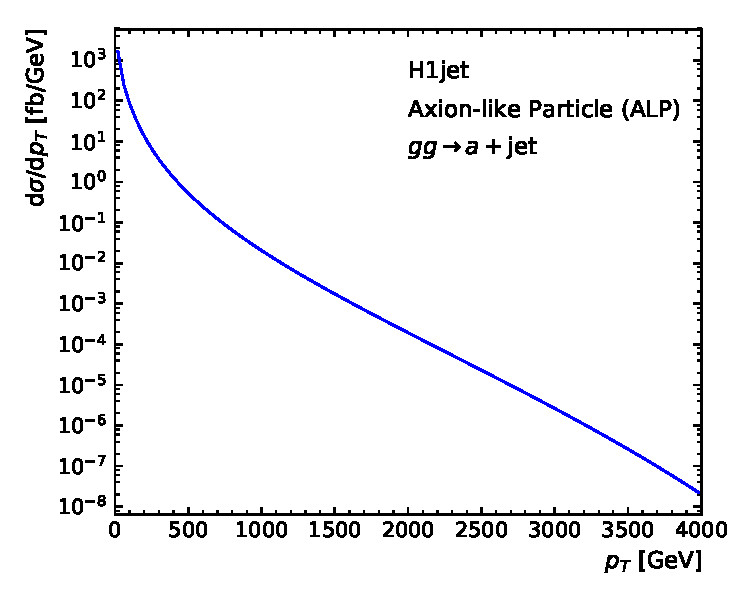
\includegraphics[width=\linewidth]{figures/ALPresult}
  \captionof{figure}{The $p_{T}$ distribution for the process $gg \rightarrow ga$ from H1jet with the amplitude from the user interface.}
  \label{fig:alpresult}
\end{minipage}%
\hfill% 
\begin{minipage}{.485\textwidth}
  \centering
  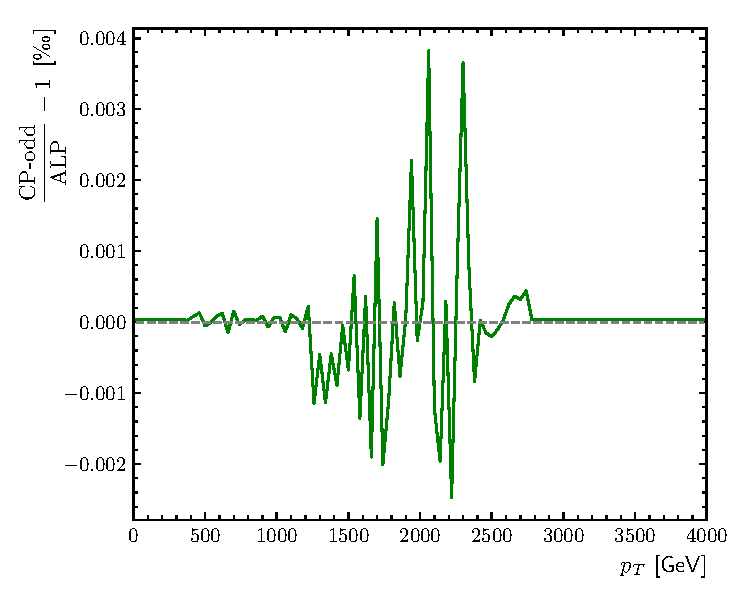
\includegraphics[width=\linewidth]{figures/ALPratio}
  \captionof{figure}{The ratio between the result from H1jet with the amplitude from \textsc{FeynCalc} and the CP-odd result.}
  \label{fig:alpratio}
\end{minipage}
\end{figure}

\subsubsection{The Total Cross-Section} \label{sec:alptotxsec} 
While not strictly necessary for the user interface to run, it is still recommended to add the code for the evaluation of the total cross-section to the custom user interface. This is easy to do as well. We will here show it for the ALP model. 

We start with considering the gluon-fusion ALP production, $gg \rightarrow a$. In Mathematica, create a tree-level $2 \rightarrow 1$ topology, and insert the fields: 
\begin{mmaCell}{Code}
tops = CreateTopologies[0, 2 -> 1];
\end{mmaCell}
\begin{mmaCell}{Code}
ins = InsertFields[tops, {V[4], V[4]} -> {S[4]}, InsertionLevel -> {Classes}, Model -> "ALP_linear_FA", GenericModel -> "ALP_linear_FA"];
\end{mmaCell}
Then set up the amplitude: 
\begin{mmaCell}{Code}
feynamp = CreateFeynAmp[ins]; 
\end{mmaCell}
\begin{mmaCell}{Code}
amp = FCFAConvert[feynamp, IncomingMomenta -> {k1, k2}, OutgoingMomenta -> {k3}, UndoChiralSplittings -> True, ChangeDimension -> 4, TransversePolarizationVectors -> {k1, k2}, List -> False, SMP -> True, Contract -> True, DropSumOver -> True] 
\end{mmaCell}
Set up the kinematics: 
\begin{mmaCell}{Code}
FCClearScalarProducts[]; 
\end{mmaCell}
\begin{mmaCell}{Code}
SP[k1, k1] = 0; 
\end{mmaCell}
\begin{mmaCell}{Code}
SP[k2, k2] = 0; 
\end{mmaCell}
\begin{mmaCell}{Code}
SP[k3, k3] = mA^2; 
\end{mmaCell}
\begin{mmaCell}{Code}
SP[k1, k2] = mA^2 / 2; 
\end{mmaCell}
Square the amplitude: 
\begin{mmaCell}{Code}
ampsquared = Simplify[
  (DoPolarizationSums[#1, k2, k1, ExtraFactor -> 1/2] & )[
    (DoPolarizationSums[#1, k1, k2, ExtraFactor -> 1/2] & )[ 
      (SUNSimplify[#1, Explicit -> True, SUNNToCACF -> False] & )[
        FeynAmpDenominatorExplicit[(1 / (SUNN^2 - 1)^2) * (amp * ComplexConjugate[amp])]]]]]
\end{mmaCell}
For a $2 \rightarrow 1$ process the parton-level cross-section is: 
\begin{equation}
	\hat{\sigma} = \frac{\pi}{s} \left \vert \mathcal{M} \right \vert^2 \delta \left ( s - m_a^2 \right ) 
\end{equation}
\begin{mmaCell}{Code}
xsec = Pi * ampsquared / mA^2 
\end{mmaCell}
Finally, write the cross-section as a Fortran code file: 
\begin{mmaCell}{Code}
Write2["ALP_xsec.f90", xsecgg = xsec, FormatType -> FortranForm, FortranFormatDoublePrecision -> False] 
\end{mmaCell}
Note here that 

\ifstandalone
\begin{thebibliography}{1}
   \bibitem{bib:h1jet} H1jet can be downloaded from: \\ \href{https://h1jet.hepforge.com}{https://h1jet.hepforge.com}
   \bibitem{bib:lhapdf} A.\ Buckley, J.\ Ferrando, S.\ Lloyd, K.\ Nordstrom, B.\ Page, M.\ Ruefenacht, M.\ Schoenherr, and G.\ Watt, \textit{LHAPDF6: parton density access in the LHC precision era}, Eur.\ Phys.\ J.\ \textbf{C75} (2015) 3, 132, [\href{https://arxiv.org/abs/1412.7420}{arXiv:1412.7420}]. 
   \bibitem{bib:hoppet} G.\ P.\ Salam and J.\ Rojo, \textit{A Higher Order Perturbative Parton Evolution Toolkit (HOPPET)}, Comput.\ Phys.\ Commun.\ \textbf{180} (2009) 120-156, [\href{https://arxiv.org/abs/0804.3755}{arXiv:0804.3755}]. 
   \bibitem{bib:chaplin} S.\ Buehler and C.\ Duhr, \textit{CHAPLIN - Complex Harmonic Polylogarithms in Fortran}, Comput.\ Phys.\ Commun.\ \textbf{185} (2014) 2703, [\href{https://arxiv.org/abs/1106.5739}{arXiv:1106.5739}]. 
   \bibitem{bib:mssm1} J.\ F.\ Gunion, H.\ E.\ Haber, \textit{The CP-conserving two-Higgs-doublet model: the approach to the decoupling limit}, Phys.\ Rev.\ D \textbf{67}, 075019 (2003), [\href{https://arxiv.org/abs/hep-ph/0207010}{arXiv:hep-ph/0207010}]. 
   \bibitem{bib:mssm2} A.\ Banfi, A.\ Bond, A.\ Martin, and V.\ Sanz, \textit{Digging for Top Squarks from Higgs data: from signal strengths to differential distributions}, J. High Energ. Phys. \textbf{2018}, 171 (2018), [\href{https://arxiv.org/abs/1806.05598}{arXiv:1806.05598}]. 
   \bibitem{bib:sushi} R.\ V.\ Harlander, S.\ Liebler, and H.\ Mantler, \textit{SusHi: A program for the calculation of Higgs production in gluon fusion and bottom-quark annihilation in the Standard Model and the MSSM}, Comput.\ Phys.\ Commun.\ \textbf{184} (2013) 1605–1617, \textbf{2018}, 171 (2018), [\href{https://arxiv.org/abs/1212.3249}{arXiv:1212.3249}]; R.\ V.\ Harlander, S.\ Liebler, and H.\ Mantler, \textit{SusHi Bento: Beyond NNLO and the heavy-top limit}, Comput.\ Phys.\ Commun.\ \textbf{212} (2017) 239–257, [\href{https://arxiv.org/abs/1605.03190}{arXiv:1605.03190}]. \\ \href{https://sushi.hepforge.org}{https://sushi.hepforge.org} 
   \bibitem{bib:feynrules} A.\ Alloul, N.\ D.\ Christensen, C.\ Degrande, C.\ Duhr, and B.\ Fuks, \textit{FeynRules 2.0 - A complete toolbox for tree-level phenomenology}, Comput.\ Phys.\ Commun.\ \textbf{185} (2014) 2250-2300, [\href{https://arxiv.org/abs/1310.1921}{arXiv:1310.1921}]. \\ \href{https://feynrules.irmp.ucl.ac.be}{https://feynrules.irmp.ucl.ac.be} 
   \bibitem{bib:alp} I.\ Brivio, M.\ B.\ Gavela, L.\ Merlo, K.\ Mimasu, J.\ M.\ No, R.\ del Rey, and V.\ Sanz, \textit{ALPs Effective Field Theory and Collider Signatures}, Eur.\ Phys.\ J.\ \textbf{C77} (2017) 572, [\href{https://arxiv.org/abs/1701.05379}{arXiv:1701.05379}]. The \textsc{FeynRules} model file is available here: \href{https://feynrules.irmp.ucl.ac.be/wiki/ALPsEFT}{https://feynrules.irmp.ucl.ac.be/wiki/ALPsEFT}. 
   \bibitem{bib:feyncalc} V.\ Shtabovenko, R.\ Mertig, and F.\ Orellana, \textit{FeynCalc 9.3: New features and improvements}, [\href{https://arxiv.org/abs/2001.04407}{arXiv:2001.04407}]; V.\ Shtabovenko, R.\ Mertig, and F.\ Orellana, \textit{New Developments in FeynCalc 9.0}, Comput.\ Phys.\ Commun.\ \textbf{64} (1991) 345-359, [\href{https://arxiv.org/abs/1601.01167}{arXiv:1601.01167}]; R.\ Mertig, M.\ Böhm, and A.\ Denner, \textit{Feyn Calc - Computer-algebraic calculation of Feynman amplitudes}, Comput.\ Phys.\ Commun.\ \textbf{64} (1991) 345-359. \\ \href{https://feyncalc.github.io}{https://feyncalc.github.io} 
   \bibitem{bib:feynarts} T.\ Hahn, \textit{Generating Feynman diagrams and amplitudes with FeynArts 3}, Comput.\ Phys.\ Commun.\ \textbf{140} (2001) 418-431, [\href{https://arxiv.org/abs/hep-ph/0012260}{arXiv:hep-ph/0012260}]. \\ \href{http://www.feynarts.de}{http://www.feynarts.de} 
   \bibitem{bib:mg5} J.\ Alwall, R.\ Frederix, S.\ Frixione, V.\ Hirschi, F.\ Maltoni, O.\ Mattelaer, H.-S.\ Shao, T.\ Stelzer, P.\ Torrielli, and M.\ Zaro, \textit{The automated computation of tree-level and next-to-leading order differential cross sections, and their matching to parton shower simulations}, [\href{https://arxiv.org/abs/1405.0301}{arXiv:1405.0301}]. \\ \href{https://launchpad.net/mg5amcnlo}{https://launchpad.net/mg5amcnlo} 
\end{thebibliography}

\end{document}
\fi
